\documentclass[a4paper,11pt]{article}

\usepackage[latin1]{inputenc}
\usepackage[T1]{fontenc}
\usepackage{bbm} %math chars
\usepackage{amsmath}
\usepackage{indentfirst}
\usepackage{fullpage} %minimizes the default margins
\usepackage{url}
\usepackage{graphicx}
\usepackage[center,footnotesize]{caption} %options des legendes des graphes
\usepackage[section]{placeins} %place les figures d'une section avant le debut de la suivante
\usepackage{subfig} %a) b) c)
\usepackage{fancyvrb}

\title{Exercises - Week 9}
\date{}
\author{Genomics and bioinformatics}

\begin{document}
\maketitle

\noindent This series is about Phylogenic Tree Reconstruction from Multiple Sequence Alignment (MSA).

\section{The Fitch's algorithm}

\noindent  Consider the following MSA:

\begin{table}[h!]
\begin{center}
\begin{tabular}{|c|c|c|c|c|}
\hline
 & 1 & 2 & 3 & 4\\
\hline
species 1 & A & C & G & T\\
\hline
species 2 & C & C & G & T\\
\hline
species 3 & A & C & C & G\\
\hline
species 4 & A & C & C & T\\
 \hline
\end{tabular}
\end{center}
\end{table}

\noindent Given a valid phylogeny tree $T$ for the above MSA (i.e.~every leaf of $T$ is labeled by a unique taxa in the MSA), the parsimony length $L(T)$ is the minimum number of mutations required to explain the tree $T$. The aim of the parsimony problem is to compute the tree $T$ which minimises $L(T)$. The tree $T$ in the following figure is the most parsimonious tree for the MSA (this tree is also found by ClustalW):

\begin{figure}[h!]
\centering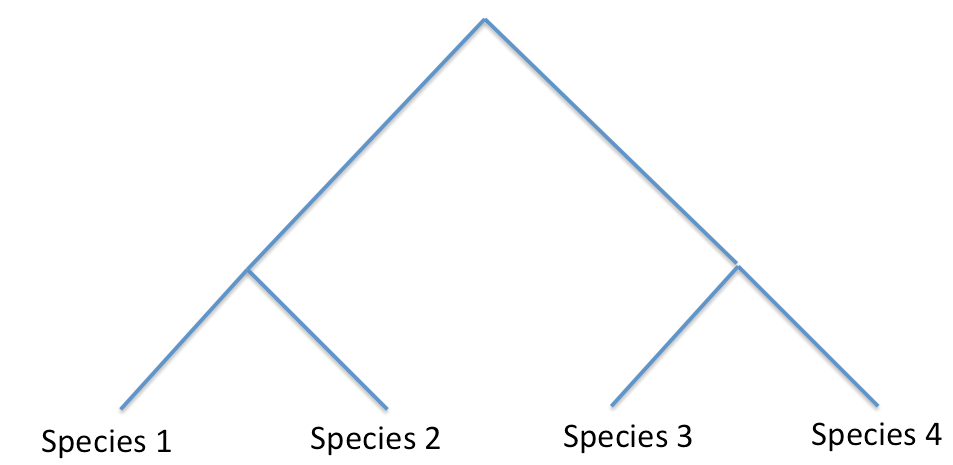
\includegraphics[width=10cm]{Tree_T.png}
\end{figure}

\noindent Assuming that the columns are independent of each other, use the Fitch's algorithm to compute the parsimony length $L(T)$ and the corresponding assignment of the states to the internal nodes. \textit{Hint:} Go from the leaves to the root (bottum-up) when applying the Fitch's algorithm and in the opposite direction (top-down) when generating the label for each internal node.

\section{The Sankoff's algorithm}

\noindent Consider the substitution matrix $M$ presented in the lectures and apply the Sankoff's algorithm to the first column of the MSA in question 1.

\section{The UPGMA algorithm}

\noindent Questions 1 and 2 used the parsimony methods. Here we shall consider the distance-based approach using the Unweighted Pair Group Method with Arithmetic mean (UPGMA) algorithm. Consider the following distance matrix:

\begin{table}[h!]
\begin{center}
\begin{tabular}{|c|c|c|c|c|c|}
\hline
 M & a & b & c & d & e\\
\hline
a & 0 & 8 & 8 & 14 & 14\\
\hline
b & 8 & 0 & 2 & 14 & 14\\
\hline
c & 8 & 2 & 0 & 14 & 14\\
\hline
d & 14 & 14 & 14 & 0 & 10\\
\hline
e & 14 & 14 & 14 & 10 & 0\\
 \hline
\end{tabular}
\end{center}
\end{table}

\noindent Use the UPGMA algorithm to build the rooted tree $T$ corresponding to the distance matrix $M$.

\end{document}











